\subsection*{Exact recovery from log-probabilities}
\label{app:exact}
\textbf{The model-specific final geometry from log-probabilities.} \Cref{thm:exact} recovers a model's own final geometry exactly from full log-probabilities. On Qwen3-0.6B ($d=1{,}024$), from 1.15 million self-generated contexts, the recovered cosines of 2{,}000 held-out contexts correlate with the true ones at \GThreeBelow\ below $d(d+1)/2$ contexts (at $0.75\times$ and $0.9\times$ the minimum-norm solution is indefinite and the recovery fails); at $1.1\times$ the correlation is \GThreeOneOne, and at $2\times$ the median error is $\GThreeErr$ (maximum $\GThreeMax$) (\cref{fig:channels}b; preregistered). Closed APIs do not return full log-probabilities.

\begin{figure}[h]
\centering
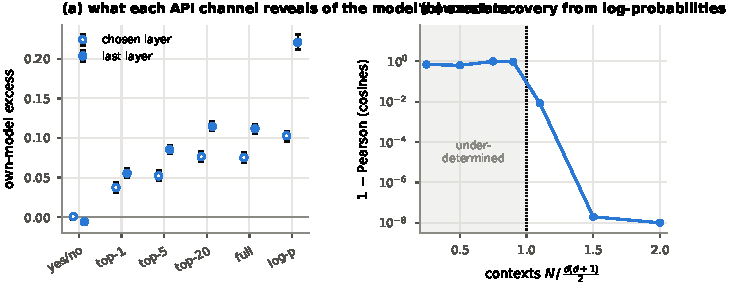
\includegraphics[width=0.8\textwidth]{figures/geometry_channels.pdf}
\caption{(a) Own-model excess for each API channel, against the last layer and the chosen layer, on 1{,}000 fresh contexts (preregistered; 95\% intervals). (b) Exact recovery of the final hidden geometry from full log-probabilities (Qwen3-0.6B, 2{,}000 held-out contexts) against the number of contexts; the threshold is $d(d+1)/2$ (preregistered).}
\label{fig:channels}
\end{figure}

Where an API returns full log-probabilities, the final state is not estimated but recovered, by the construction of \citet[App.~H]{carlini2024stealing}.
\begin{theorem}[exact recovery; after Carlini et al.]\label{thm:exact}
Let the logits be $Wu$, with $u=x/\mathrm{rms}(x)$ the normalised final state, the normalisation gain folded into $W$, and no output bias. The centred log-probabilities $c(x)$ lie in a $d$-dimensional subspace; write $b=Q_d^{\top}c$ for an orthonormal basis $Q_d$ of it. Then $u=Kb$ for an unknown invertible $K$, and $\|u\|^2=d$ gives $b_i^{\top}Sb_i=d$ with $S=K^{\top}K$: a linear system in $S$. If the $b_ib_i^{\top}$ span the symmetric matrices (generically, $N\ge d(d+1)/2$ contexts), $S$ is unique, and the Gram matrix of the final states, $b_i^{\top}Sb_j=u_i^{\top}u_j$, is exact for every new context. The states follow up to an orthogonal map: the gauge group.
\end{theorem}
The subspace \citep{finlayson2024logits} and the ellipsoid fit that removes all but an orthogonal ambiguity \citep[App.~H]{carlini2024stealing} are known; we state the consequence for the gauge-invariant geometry and test its sharp transition at $d(d+1)/2$ contexts. Recovery holds up to the normalisation's $\epsilon$, and near the threshold the system is badly conditioned.

\subsection{The observable geometry}
\begin{proof}[Proof of \cref{thm:geometry}]
(a) The Fisher information of $\mathrm{Bernoulli}(p)$ is $1/(p(1-p))$ and $\mathrm{d}\vartheta/\mathrm{d}p=1/\sqrt{p(1-p)}$, so the metric is $\mathrm{d}\vartheta^2$. The Fisher metric of a product of independent factors is the sum of the factors' metrics, so in $\vartheta$ the family is the box $[0,\pi]^m$ with the Euclidean metric. The box is convex, so geodesics are segments and the distance is Euclidean. Check for one factor: the Bhattacharyya coefficient of $\mathrm{Bernoulli}(\sin^2\alpha)$ and $\mathrm{Bernoulli}(\sin^2\beta)$ is $\cos(\alpha-\beta)$, and $2\arccos\cos(\alpha-\beta)=|\vartheta-\vartheta'|$.
(b) Invariance: $d_Q$ is a function of $(P_x,P_{x'})$ only, and \cref{prop:gauge} leaves every output law unchanged. Uniqueness of the Fisher metric on the simplex over the finite set $\{0,1\}^m$, under Markov morphisms, is \v{C}encov's theorem. $d_Q$ is the intrinsic geodesic distance of the submanifold of independent laws; the geodesic distance of the whole simplex between two product laws is $2\arccos$ of their Bhattacharyya coefficient, $2\arccos\prod_j\cos\frac{\vartheta_j-\vartheta'_j}{2}$, which is a different function of the same angles.
(c) $\mathrm{d}\vartheta_j=\Psi_j'/\sqrt{\Psi_j(1-\Psi_j)}$ and $\Psi_j'=\Psi_j(1-\Psi_j)\nabla a_j^{\top}\Delta$, so $\mathrm{d}\vartheta_j=\sqrt{\Psi_j(1-\Psi_j)}\,\nabla a_j^{\top}\Delta$; summing the squares gives $\Delta^{\top}G_Q\Delta$, and the remainder is third order by Taylor's theorem.
(d) $\hat\vartheta$ is increasing in $k$ and $k$ is stochastically increasing in $p$, so $\mu_n$ is strictly increasing; $\mu_n\to\vartheta$ by the law of large numbers and continuity. The halves are independent, so $\E[(a_A-a'_A)(a_B-a'_B)]=(\E a_A-\E a'_A)(\E a_B-\E a'_B)=(\mu_n(\Psi)-\mu_n(\Psi'))^2$ for each question; sum over questions. This needs the same $n$ in every cell: with $n_A(x)\ne n_A(x')$ the factor is $\mu_{n_A(x)}(\Psi)-\mu_{n_A(x')}(\Psi')$, not a difference of one function. Clipping a negative $\hat D^2$ at $0$, as needed for distances, adds a non-negative bias. Classical scaling recovers a Euclidean configuration from its distance matrix up to a rigid motion (Young--Householder; Torgerson). Note that the familiar large-$n$ variance $1/(n+\frac12)$ of the Anscombe angle fails near $p\in\{0,1\}$ and its bias is $\cot\vartheta/(4n)$, so subtracting a variance term is not exact; the cross-fit needs neither.
\end{proof}
\begin{proof}[Proof of \cref{thm:exact}]
With $P=I-\mathbf{1}\mathbf{1}^{\top}/V$, the log-softmax removes a constant per context, so $c=PWu$ and every $c$ lies in the column space of $PW$, of dimension $d$ when $PW$ has full column rank. Let $Q_d$ be an orthonormal basis of it and $b=Q_d^{\top}c=Mu$ with $M=Q_d^{\top}PW$ invertible; then $u=Kb$ with $K=M^{-1}$. $\|u\|^2=b^{\top}K^{\top}Kb=d\,\overline{x^2}/(\overline{x^2}+\epsilon)$, which is $d$ up to the normalisation's $\epsilon$. The map $S\mapsto(b_i^{\top}Sb_i)_i$ is linear on the $d(d+1)/2$-dimensional space of symmetric matrices; it is injective iff the $b_ib_i^{\top}$ span that space, which for $b_i$ in general position needs and generically holds with $N\ge d(d+1)/2$. Then $S=K^{\top}K$ is the unique solution and $B^{\top}SB=U^{\top}U$. Any $L$ with $L^{\top}L=S$ satisfies $L=OK$ for an orthogonal $O$, so the states are fixed up to $O$, the group of \cref{prop:gauge}.
\end{proof}

\textbf{The variance-subtraction rule is not exact (Correction 1).} Our locked theory first stated that $\|\hat\vartheta(x)-\hat\vartheta(x')\|^2-2m/(n+\frac12)$ is unbiased up to $O(mn^{-2})$. Exact binomial sums show that the bias of $\hat\vartheta$ is $\cot\vartheta/(4n)+O(n^{-2})$ (at $n=32$: $0.0102$ vs $0.0104$ at $p=0.1$), that the variance is below $1/(n+\frac12)$ near $p\in\{0,1\}$ ($0.68/(n+\frac12)$ at $p=0.1$, $n=8$), and that with $n$ samples the angles cannot leave $[2\arcsin\sqrt{(3/8)/(n+3/4)},\,\pi-2\arcsin\sqrt{(3/8)/(n+3/4)}]$, so large distances between saturated answers contract. The cross-fit of \cref{thm:geometry}(d) replaces the rule; the preregistered endpoints used the locked rule as specified and are reported as such. On Claude Haiku 5.5 the cross-fit lowers the negative eigenvalue mass of classical scaling from \CFClosedANeg\ to \CFClosedANegCF; on open models it keeps the same rank agreement with the hidden geometry (exploratory).

\textbf{The solver.} We whiten $b$ on the training contexts (any invertible map of $b$ is allowed) and solve the least-squares problem for symmetric $S$ by conjugate gradient on the normal equations, from $S=0$, which gives the minimum-norm solution when $N<d(d+1)/2$. On synthetic heads with known $K$ ($d=16,48$) the cosine error is $10^{-10}$ to $10^{-12}$ above the threshold and $0.04$--$0.09$ below it.

